\chapter{Introduction}
\label{chapter:introduction}

The neural circuits of the brain are wired into a complex network \cite{sporns2010networks}. 
Collective signalling within this network manifests as patterned neural activity, 
and these emergent dynamics are thought to support the computations that underlie cognition 
and adaptive behaviour \cite{gerstner1945neuronal,chialvo2010emergent,ju2020dynamic}. Recent technological 
advances have enabled increasingly comprehensive reconstructions of biological brain networks 
\cite{vanessen2012human,glasser2016human,elam2021human}. 
These maps, termed connectomes \cite{sporns2005human,sporns2011human,sporns2013human}, 
display a range of non-random architectural features, including heavy-tailed degree distributions 
\cite{hagmann2008mapping,sporns2007identification}, segregated communities 
\cite{betzel2017modular,bertolero2015modular,power2011functional} and a densely interconnected core 
\cite{zamora2010cortical,van2012high,towlson2013rich}. 
A growing body of work suggests that these topological attributes enhance the network's capacity 
to process information \cite{van2016comparative,bassett2017network}. Despite these insights, how macroscale connectivity gives rise to the 
computational properties of the activity it supports remains poorly understood.

We hypothesise that structure shapes computation. Specifically, we propose that the human connectome 
governs the computational properties of the dynamics it produces, and we aim to characterise the 
mechanisms underlying this relationship. Structure and computation sit far apart: a wiring diagram 
is a static object, whereas computation is a property of activity unfolding in time. Rather than 
mapping one directly onto the other, we proceed through two intermediate steps. The first is the 
eigenspectrum of the connectivity matrix, which is derived from the wiring alone yet already 
describes how activity behaves \cite{rajan2010stimulus,christodoulou2022eigenvalue}. 
The second is the geometry of the activity itself, the shape traced out by the network's response 
to the inputs it receives \cite{ju2020dynamic,vyas2020computation}. Structure sets the spectrum, 
the spectrum shapes the geometry of activity, and that geometry governs what the network can compute.

Reservoir computing offers a way to follow this chain \cite{lukovsevivcius2009reservoir}. 
Introduced as a machine learning framework for training recurrent networks efficiently 
\cite{jaeger2001echo,maass2002real}, it has been adopted increasingly widely for connectome-constrained 
models \cite{suarez2024connectome,suarez2021learning,milisav2026neuromorphic,damicelli2022brain}. 
A recurrent neural network (RNN) of nonlinear units is paired with a linear readout, and only 
the readout is trained. The recurrent weights are fixed, which allows us to impose an arbitrary 
connectivity pattern and know that it survives learning intact. Network structure is therefore isolated 
as the single feature under investigation, and the dynamics, being determined by the fixed wiring, 
can be tuned and held wherever we choose. We use this framework to construct recurrent networks endowed 
with connection patterns derived from diffusion-weighted imaging of human brains \cite{griffa2019structural}.

The eigenvalues of such a network describe how activity evolves once it is perturbed: how quickly each 
pattern fades or persists, and whether it rotates to produce oscillations \cite{lehmann1991eigenvalue, rajan2006eigenvalue}. 
This turns a static wiring diagram into a description of the timescales and rhythms a network can support, 
precisely the properties computations rely on. 
Two parts of the spectrum play distinct roles. The largest eigenvalue acts as an 
overall gain, a single number scaling how strongly the network responds to what it is given, and with 
it the dynamical regime the network occupies. The eigenvalues beneath it are where a network's 
particular wiring leaves its mark. How far the largest stands apart from the rest is central to what 
we find. Separating these two roles is essential to our approach: the first is a property we control, 
and the second is the property we study.

To connect these dynamics to computation, we examine the geometry of the activity a network produces. 
When a network is driven by an input, its units do not all respond in the same way: the pattern of 
activity moves around, and the shape of that movement can be described geometrically 
\cite{chung2021neural,clark2025connectivity}. 
One might reasonably expect that a network whose activity spreads widely retains more of what it was given 
\cite{clark2023dimension,gao2017theory}. If activity is confined to a few directions, there is little for a readout to work with, 
whereas if it fluctuates more broadly, more of the input's history should remain recoverable.
This is not what we find. The directions in which activity varies most carry little that a readout 
can use, while the information a readout can recover lies in directions so faint they are easily mistaken 
for noise. What matters is not how widely activity spreads, but how many independent directions remain 
available to a readout, however small their contribution to the network's overall movement. 
This reversal recurs throughout the report, and it is why we track the shape of activity rather than 
its magnitude.

These connectome-constrained reservoirs are trained on two families of task: memory and prediction. 
Memory reflects a network's ability to retain information, while prediction reflects its ability to 
generate new information conditioned on what it has seen. We take these to be two fundamental properties 
of a computational system, and cornerstones of the brain's capacity to process information and support 
cognition \cite{bar2009proactive}. They are not, however, two views of the same quantity. 
Memory and prediction respond differently to the same structural manipulations, and much of what 
follows concerns the terms on which one is traded against the other.

Testing our hypothesis requires comparing the connectome against alternative network variants, referred 
to as null models \cite{vavsa2022null}. Null models provide a flexible tool for benchmarking the presence 
or magnitude of a feature of interest, by selectively preserving certain architectural properties of a 
network while systematically randomising others. 
Here we assess both the memory and the predictive capacity of 
empirically derived connectomes against five null models, which form a ladder that isolates the 
properties that may shape their capacity. These include topological attributes such as edge density, 
degree sequence, modularity and clustering. Throughout the report we focus in particular on edge 
weights, the strength of connections, and on how their magnitude, sign and assignment shape a network's 
activity. Sign warrants a caveat. The macroscale connectome reconstructed from diffusion imaging is 
non-negative by construction \cite{behrens2012human}, since streamline counts cannot be negative, 
so introducing negative weights is a controlled counterfactual rather than a reconstruction of anatomy. 
We treat it as such, and distinguish throughout between manipulations applied edge by edge, 
which serve as a mechanistic control, and manipulations applied node by node, which respect the 
constraint that a neuronal population is predominantly excitatory or inhibitory and therefore carry 
the biological interpretation.

Finally, we investigate how computational capacity depends on the dynamical state of the network. To 
evaluate the contributions of structure and dynamics, we parametrically tune this state, driving the 
network between stable, critical and chaotic regimes \cite{kadmon2015transition}. 
These regimes describe what a network does with what it is given: in the stable regime activity dies 
away quickly and little of the input is retained, in the chaotic regime activity is amplified until 
the response is dominated by the network's own noise \cite{sompolinsky1988chaos}, 
and between the two lies a critical regime where inputs persist long enough to be useful without being 
destroyed. Previous work has shown that biologically realistic architectures perform best when their 
dynamics are critical \cite{bertschinger2004edge}, which raises the question of how a biological network comes to occupy and hold 
such a state.
This returns us to the eigenspectrum, since the leading eigenvalue sets the gain and with it the regime. 
Rescaling it places different networks at comparable operating points, and doing so is what makes a fair 
comparison across structures possible: without it, differences in performance would reflect little more 
than differences in overall gain \cite{suarez2021learning}. A network's capability is therefore not a single number but a curve, 
measured across the range of dynamical states it can occupy. What is held fixed in constructing that 
curve is itself consequential, and we treat this as a question to be examined rather than a convention 
to be applied. 

This report traces the mechanisms that link structure to spectrum, spectrum to the geometry of activity, 
and geometry to what a network can compute. Followed through in this way, differences in wiring cease to 
be descriptive facts and acquire consequences. Together these begin to explain how the organisation of 
the brain supports computation, with implications for both neuroscience and artificial intelligence 
\cite{hassabis2017neuroscience,sadeh2025emergence}.


% Discoveries box
\clearpage
\begin{contributions}[Discoveries and contributions]
    \item \textbf{The connectome's spectrum is distinguished by a gap, not by a
    compressed bulk.} Its largest eigenvalue stands unusually far apart from the
    rest, while the remainder of the spectrum is close to that of every null
    model we test. The effect is traced to where the strong connections sit,
    rather than to the network's topology or to the distribution of weights
    taken on its own.

    \item \textbf{What a readout can use is not where the activity is largest.}
    Memory is carried by many faint directions of activity, which measures
    weighted by variance discount almost entirely. The dimensionality of neural
    activity is meaningful only relative to what reads it out.

    \item \textbf{The connectome's memory advantage is retention, not peak
    capacity.} At its best operating point it performs on a par with its nulls,
    or marginally below. What distinguishes it is how much of that performance
    survives as the network is driven away from that point, which its spectral
    gap protects by keeping activity from being swamped by a single dominant
    mode.

    \item \textbf{Predictive capacity is gated by dynamical regime rather than
    graded by geometry.} Introducing inhibitory connections brings a second
    dynamical branch within reach, and networks fall into one regime or the
    other rather than varying smoothly between them. Across a biologically
    plausible range of inhibition, the connectome is the only network still
    predicting usefully.

    \item \textbf{Memory and prediction trade against one another along a single
    structural axis.} The property that holds a trajectory smooth enough to be
    continued is the same one that synchronises units and consumes the
    directions a readout would otherwise use. The two advantages therefore
    occupy opposite regions of the same parameter space.

    \item \textbf{How networks are matched for comparison is not a neutral
    choice.} These networks differ in essentially one spectral quantity, so any
    convention for equating them fixes part of the mechanism under test. Every
    claim here is reported under both conventions and rests on surviving both. \\

Together these suggest a way of reading the brain's structure that complements the 
usual one: less as an arrangement that maximises what a network can compute, and 
more as one that reduces how precisely it must be tuned in order to compute at all.

\end{contributions}


% Overview schematic
\begin{figure}[ht]
    \centering
    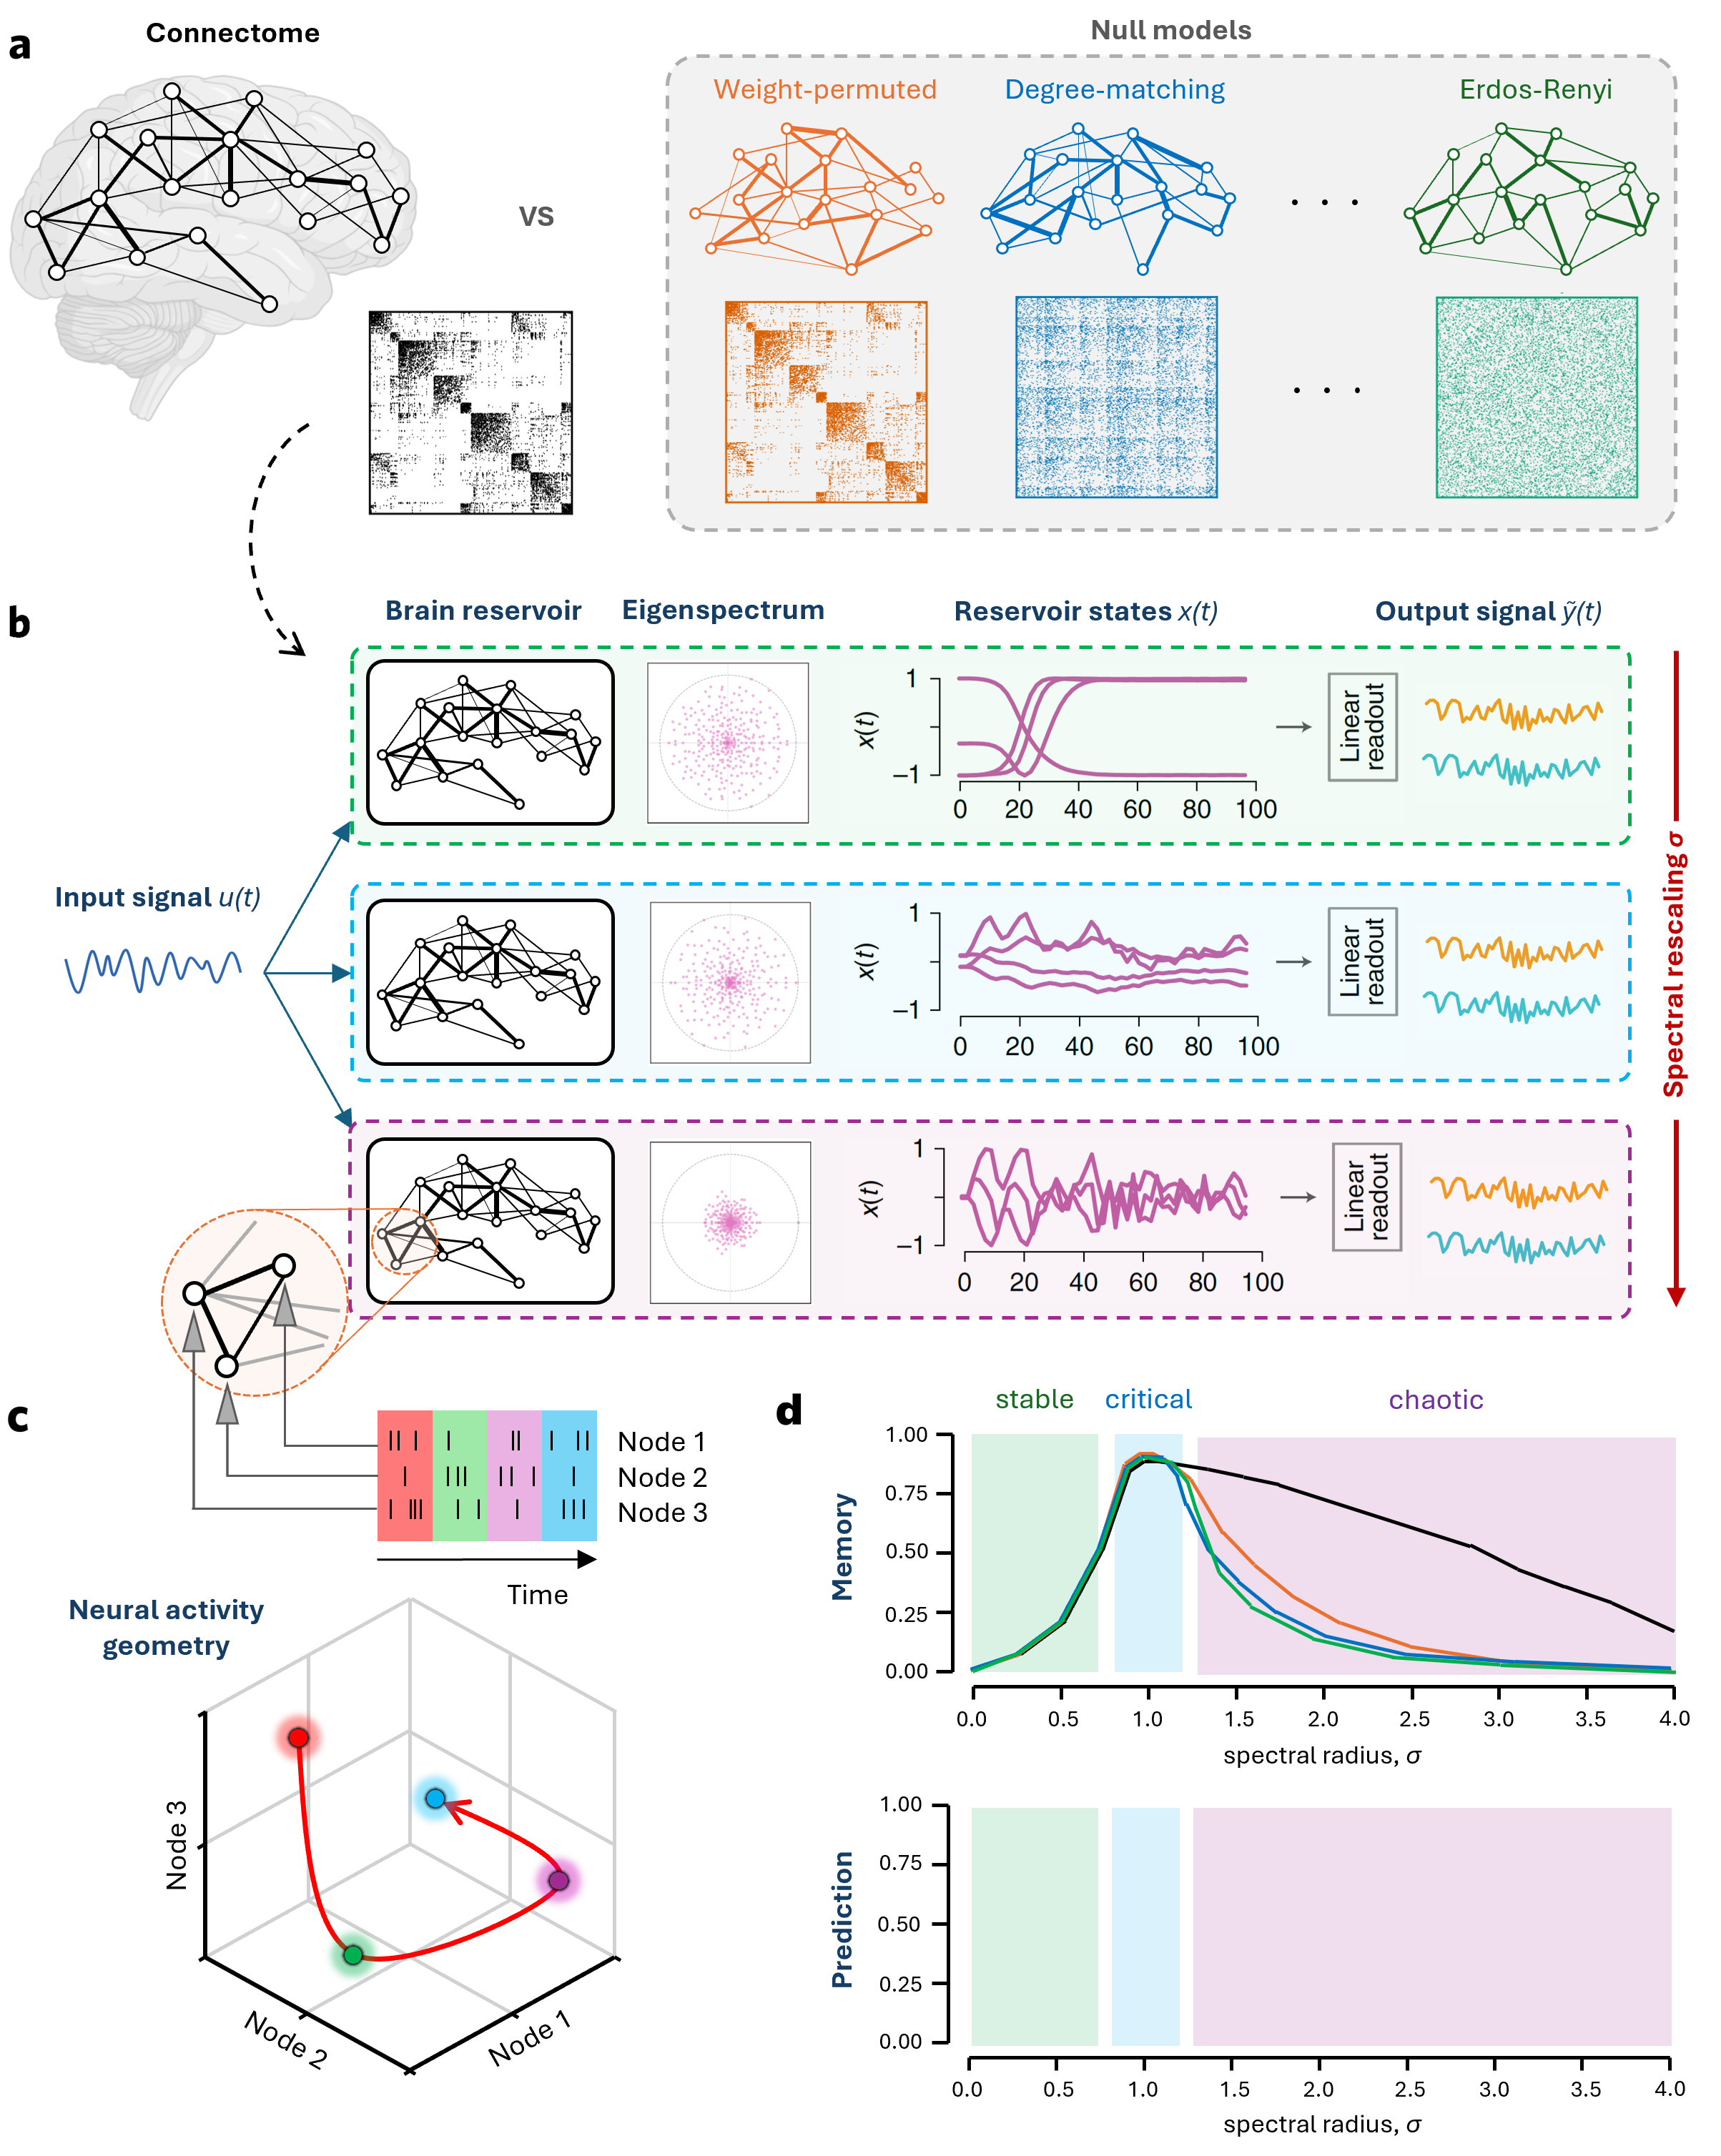
\includegraphics[width=\textwidth]{figures/Intro-Schematic.png}
    \caption[Main fig]{
    \textbf{Overview schematic:} Caption to be written soon...}
    \label{fig:project-schematic}
\end{figure}


\afterpage{\blankpage}
